\resizebox{0.8\columnwidth}{!}{
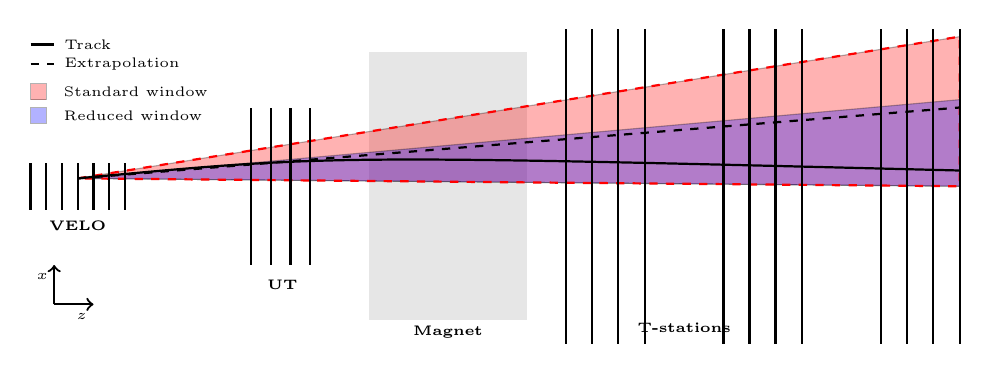
\begin{tikzpicture}
  %\draw[step=1cm,gray,very thin] (0,0) grid (12,4);

  \fill[gray,opacity=0.2] (4.5,0.3) rectangle (6.5,3.7);
  \node[draw=none] at  (5.5,0.15){\tiny \bf{Magnet}};

  \draw[fill=red,opacity=0.3] (0.8,2.1) -- (12.0,3.9) -- (12.0,2.0)--cycle;
  \draw[fill=blue,opacity=0.3] (0.8,2.1) -- (12.0,3.1) -- (12.0,2.0)--cycle;
  \draw[color=red,dashed,thick] (0.8,2.1) -- (12.0,3.9) -- (12.0,2.0)--cycle;

  %VELO
  \node[draw=none] at  (0.8,1.5){\tiny \bf{VELO}};
  \draw[thick] (0.2,1.7) -- (0.2,2.3);
  \draw[thick] (0.4,1.7) -- (0.4,2.3);
  \draw[thick] (0.6,1.7) -- (0.6,2.3);
  \draw[thick] (0.8,1.7) -- (0.8,2.3);
  \draw[thick] (1.0,1.7) -- (1.0,2.3);
  \draw[thick] (1.2,1.7) -- (1.2,2.3);
  \draw[thick] (1.4,1.7) -- (1.4,2.3);

  %TT
  \node[draw=none] at  (3.4,0.75){\tiny \bf{UT}};
  \draw[thick] (3.0,1.0) -- (3.0,3.0);
  \draw[thick] (3.25,1.0) -- (3.25,3.0);
  \draw[thick] (3.5,1.0) -- (3.5,3.0);
  \draw[thick] (3.75,1.0) -- (3.75,3.0);

  %T
  \node[draw=none] at  (8.5,0.2){\tiny \bf{T-stations}};
  \draw[thick] (7.0,0.0) -- (7.0,4.0);
  \draw[thick] (7.33,0.0) -- (7.33,4.0);
  \draw[thick] (7.66,0.0) -- (7.66,4.0);
  \draw[thick] (8.0,0.0) -- (8.0,4.0);

  \draw[thick] (9.0,0.0) -- (9.0,4.0);
  \draw[thick] (9.33,0.0) -- (9.33,4.0);
  \draw[thick] (9.66,0.0) -- (9.66,4.0);
  \draw[thick] (10.0,0.0) -- (10.0,4.0);

  \draw[thick] (11.0,0.0) -- (11.0,4.0);
  \draw[thick] (11.33,0.0) -- (11.33,4.0);
  \draw[thick] (11.66,0.0) -- (11.66,4.0);
  \draw[thick] (12.0,0.0) -- (12.0,4.0);

  \draw[thick,dashed] (0.8,2.1) -- (12,2+10*0.1);
  \draw[thick] (0.8,2.1) .. controls (4,2.4) .. (12,2.2);

  \draw[thick] (0.2,3.8) -- (0.5,3.8)  node[anchor=west] {\tiny Track};
  \draw[thick,dashed] (0.2,3.55) -- (0.5,3.55)  node[anchor=west] {\tiny Extrapolation};
  \draw[white] (0.2,3.2) -- (0.5,3.2)  node[anchor=west] {\tiny \textcolor{black}{Standard window}};
  \draw[white] (0.2,2.9) -- (0.5,2.9)  node[anchor=west] {\tiny \textcolor{black}{Reduced window}};
  \draw[fill=red,opacity=0.3] (0.2,3.1) rectangle (0.4,3.3);
  \draw[fill=blue,opacity=0.3] (0.2,2.8) rectangle (0.4,3.0);
  %\node[draw=none] at  (1.5,3.2){\tiny Standard window};
  %\node[draw=none] at  (1.5,2.9){\tiny Reduced window};

  \draw[thick,->] (0.5,0.5) -- (0.5,1.0);
  \draw[thick,->] (0.5,0.5) -- (1.0,0.5);
  \node[draw=none] at (0.35,0.85){\tiny $x$};
  \node[draw=none] at (0.85,0.35){\tiny $z$};

  

\end{tikzpicture}
}
